\documentclass[11pt,compress,t,notes=noshow, aspectratio=169, xcolor=table]{beamer}

\usepackage{../../style/lmu-lecture}
% Defines macros and environments
% This file is included in slides and exercises

% Rarely used fontstyle for R packages, used only in 
% - forests/slides-forests-benchmark.tex
% - exercises/single-exercises/methods_l_1.Rnw
% - slides/cart/attic/slides_extra_trees.Rnw
\newcommand{\pkg}[1]{{\fontseries{b}\selectfont #1}}

% Spacing helpers, used often (mostly in exercises for \dlz)
\newcommand{\lz}{\vspace{0.5cm}} % vertical space (used often in slides)
\newcommand{\dlz}{\vspace{1cm}}  % double vertical space (used often in exercises, never in slides)
\newcommand{\oneliner}[1] % Oneliner for important statements, used e.g. in iml, algods
{\begin{block}{}\begin{center}\begin{Large}#1\end{Large}\end{center}\end{block}}

% Don't know if this is used or needed, remove?
% textcolor that works in mathmode
% https://tex.stackexchange.com/a/261480
% Used e.g. in forests/slides-forests-bagging.tex
% [...] \textcolor{blue}{\tfrac{1}{M}\sum^M_{m} [...]
% \makeatletter
% \renewcommand*{\@textcolor}[3]{%
%   \protect\leavevmode
%   \begingroup
%     \color#1{#2}#3%
%   \endgroup
% }
% \makeatother


\tikzset{main node/.style={rectangle,draw,minimum size=1cm,inner sep=4pt},}

\title{Interpretable Machine Learning}
% \author{LMU}
%\institute{\href{https://compstat-lmu.github.io/lecture_iml/}{compstat-lmu.github.io/lecture\_iml}}
\date{}

\def\firstrowcolor{}
\def\secondrowcolor{}
\def\thirdrowcolor{}
\def\fourthrowcolor{}

\begin{document}

\newcommand{\titlefigure}{figure/tree_surface2.png}
\newcommand{\learninggoals}{
% \item Model-based boosting with simple base learners
% \item Feature effect and importance in model-based boosting}
\item Decision trees
\item RuleFit
\item Decision rules}

\lecturechapter{Rule-based Models}
\lecture{Interpretable Machine Learning}

\begin{frame}{Decision Trees \citebutton{Breiman et al. (1984)}{https://doi.org/10.1201/9781315139470}}

%\textbf{Problem}: Can we model non-linear effects and interactions automatically (without manual specification as in GLMs or GAMs)?\\
%Relationship between features and target are non-linear or interactions are present\\
%\medskip
%\pause

\textbf{Idea}: 
%Split data in different subsets based on cut-off values in features 
Partition data into axis-aligned regions via greedy search for feature cut points (minimizing a split criterion), then predict a constant mean $c_m$ in each leaf region $\mathcal{R}_m$:
%Partition data into subsets based on cut-off values in features (found by minimizing a split criterion via greedy search) and predict constant mean $c_m$ in leaf node $\mathcal{R}_m$:

\begin{columns}[T, totalwidth=\textwidth]

\begin{column}{0.65\textwidth}
$$
\textstyle\hat f(x) = \sum\limits_{m=1}^M c_m \mathds{1}_{\{x \in \mathcal{R}_m\}}
$$

% \begin{itemize}
% \item where $c_m$ is a constant and 
% \item $\mathcal{R}_m$ the $m$-th leaf node of the tree
% \end{itemize}
\pause
\begin{itemize}
    %\item Finding best split point (CART): Greedy search for the point that minimizes the variance of $y$ (regression) or the Gini index (classification)
    \item Applicable to regression and classification
    \item Models interactions and non-linear effects
    \item Handles mixed feature spaces \& missing values
\end{itemize}

\end{column}
\begin{column}{0.35\textwidth}
\vspace{0.15cm}
\centering
\begin{tikzpicture}[scale=0.8, transform shape]
   \usetikzlibrary{arrows}
    \usetikzlibrary{shapes}
     \tikzset{treenode/.style={draw, circle, font=\small}}
     \tikzset{line/.style={draw, thick}}
     \node [treenode, draw=red] (a0) {};
     \node [treenode, below=0.75cm of a0, xshift=-1.5cm]  (a1) {};
     \node [treenode, below=0.75cm of a0, xshift=1.5cm]  (a2) {};

     \node [treenode, below=0.75cm of a2, xshift=-0.75cm] (a3) {$c_1$};
     \node [treenode, below=0.75cm of a2, xshift=0.75cm]  (a4) {$c_2$};

    \node [treenode, below=0.75cm of a1, xshift=-0.75cm] (a5) {$c_3$};
    \node [treenode, below=0.75cm of a1, xshift=0.75cm]  (a6) {$c_4$};

     \path [line] (a0.south) -- + (0,-0.4cm) -| (a1.north) node [midway, above] {$x_1<3$};
     \path [line] (a0.south) -- +(0,-0.4cm) -|  (a2.north) node [midway, above] {$x_1\geq3$};

     \path [line] (a2.south) -- + (0,-0.4cm) -| (a3.north) node [midway, above] {$x_2<6$};;
     \path [line] (a2.south) -- +(0,-0.4cm) -|  (a4.north) node [midway, above] {$x_2\geq6$};

    \path [line] (a1.south) -- + (0,-0.4cm) -| (a5.north) node [midway, above] {$x_3<2$};;
    \path [line] (a1.south) -- +(0,-0.4cm) -|  (a6.north) node [midway, above] {$x_3\geq2$};

    %\path (a5.south) -- +(0,0) -|  (a5.south) node [midway, below] {$f_{1,3}(x_1,x_3)$};
    %\path (a6.south) -- +(0,0) -|  (a6.south) node [midway, below] {$f_{1,3}(x_1,x_3)$};

    %\path (a3.south) -- +(0,0) -|  (a3.south) node [midway, below] {$f_{1,2}(x_1,x_2)$};
    %\path (a3.south) -- +(0,0) -|  (a4.south) node [midway, below] {$f_{1,2}(x_1,x_2)$};
    % \path (a3) edge [bend right, draw=white] node [below] {$f_{1,2}(x_1,x_2)$} (a4);
    % \path (a5) edge [bend right, draw=white] node [below] {$f_{1,3}(x_1,x_3)$} (a6);
   \end{tikzpicture}
   
\end{column}
\end{columns}
%\vspace{-0.4cm}
\begin{center}
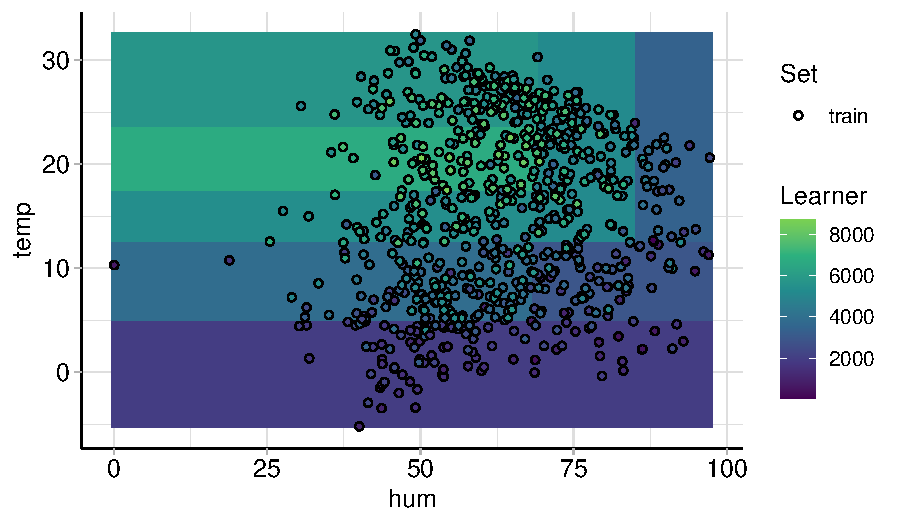
\includegraphics[width=0.45\textwidth]{figure/tree_surface1.pdf} \qquad  
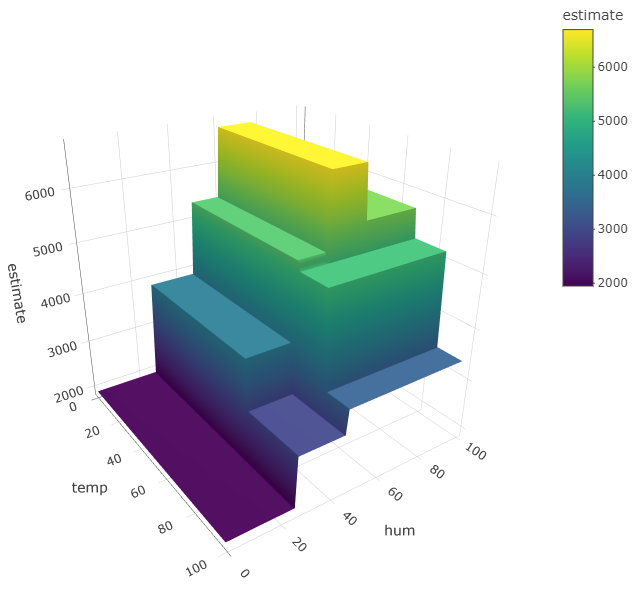
\includegraphics[width=0.33\textwidth]{figure/tree_surface2.png}
\end{center}

\end{frame}


% \begin{frame}{Interpretation}
% \begin{itemize}
%     \item Directly by following the tree structure (i.e., sequence of decision rules)
%     \item Importance of $x_j$: Aggregate ``improvement in split criterion'' over all splits where $x_j$ was involved\\
%     \item[] $\leadsto$ e.g., variance for regression or Gini index for classification
%     %Feature importance: How much did split criterion improve compared to parent node% by (scaled) score of how much splitting criterion (e.g. variance) is reduced compared to a parent node
% \end{itemize}

% \end{frame}

\begin{frame}{Interpretation of Tree-Based Models}
\begin{itemize}
    \item Interpretation via path of decision rules along tree branches
    \item \textbf{Feature importance} (quantifies how often and how usefully $x_j$ is used): 
    \begin{itemize}
        \item For each split on feature $x_j$, record the decrease in the split criterion 
        \item Aggregate this over the tree: sum or average over all splits involving $x_j$
        \item Split criterion: variance (regression), Gini index / entropy (classification)
    \end{itemize}
    %\item[] $\leadsto$ Quantifies how often and how usefully $x_j$ is used
\end{itemize}
\begin{columns}[T, totalwidth=\textwidth]
  \begin{column}{0.6\textwidth}
    %\begin{center}
    % \begin{tikzpicture}[scale=0.7, every node/.style={font=\small}]
    %   % Nodes
    %   \node[draw, circle] (root) at (0,0) {$x_j < 5$};
    %   \node[draw, circle] (left) at (-3,-2.5) {$x_k < 3$};
    %   \node[draw, rectangle] (L1) at (-4.2,-5) {$c_1$};
    %   \node[draw, rectangle] (L2) at (-1.8,-5) {$c_2$};

    %   \node[draw, circle] (right) at (3,-2.5) {$x_k < 7$};
    %   \node[draw, rectangle] (R1) at (2,-5) {$c_3$};
    %   \node[draw, rectangle] (R2) at (4,-5) {$c_4$};

    %   % Edges with labels
    %   \draw[->] (root) -- node[above left] {\scriptsize } node[midway, left=3pt] {\scriptsize  $\Delta\text{Var} = 0.18$} (left);
    %   \draw[->] (root) -- node[above right] {\scriptsize } node[midway, right=3pt] {\scriptsize } (right);

    %   \draw[->] (left) -- node[left] {\scriptsize $\Delta\text{Var} = 0.07$} (L1);
    %   \draw[->] (left) -- (L2);

    %   \draw[->] (right) -- node[left] {\scriptsize $\Delta\text{Var} = 0.10$} (R1);
    %   \draw[->] (right) -- (R2);
    % \end{tikzpicture}
    \begin{tikzpicture}[scale=0.75, every node/.style={font=\small}]
  % Nodes: rectangular with split condition + delta
  \node[draw, ellipse, align=center] (root) at (0,0) {$x_j < 5$\\ \scriptsize$ \Delta\text{Var} = 0.18$};
  \node[draw, ellipse, align=center] (left) at (-3,-2.5) {$x_k < 3$\\ \scriptsize$\Delta\text{Var} = 0.07$};
  \node[draw, ellipse, align=center] (right) at (3,-2.5) {$x_k < 7$\\ \scriptsize$\Delta\text{Var} = 0.10$};

  % Leaf nodes
  \node[draw, rectangle] (L1) at (-4.2,-5) {$c_1$};
  \node[draw, rectangle] (L2) at (-1.8,-5) {$c_2$};
  \node[draw, rectangle] (R1) at (2,-5) {$c_3$};
  \node[draw, rectangle] (R2) at (4,-5) {$c_4$};

  % Edges (unlabeled)
  \draw[->] (root) -- (left);
  \draw[->] (root) -- (right);
  \draw[->] (left) -- (L1);
  \draw[->] (left) -- (L2);
  \draw[->] (right) -- (R1);
  \draw[->] (right) -- (R2);
\end{tikzpicture}

    %\end{center}
  \end{column}

  \begin{column}{0.4\textwidth}
    \begin{itemize}
  \item Each $\Delta\text{Var}$ is assigned to the splitting feature
  % Variance reductions $\Delta\text{Var}$ from splits are attributed to the splitting feature.
  \item Feature importance = sum of all $\Delta\text{Var}$ for that feature:
  \begin{itemize}
    \item[$x_j$:]  $0.18$
    \item[$x_k$:]  $0.07 + 0.10 = 0.17$
  \end{itemize}
    \end{itemize}
  \end{column}
\end{columns}
% \vspace{0.4cm}
% \begin{center}
% \begin{tikzpicture}[scale=0.7, every node/.style={font=\small}]
%   % Nodes
%   \node[draw, circle] (root) at (0,0) {$x_j < 5$};
%   \node[draw, circle] (left) at (-3,-2.5) {$x_k < 3$};
%   \node[draw, rectangle] (L1) at (-4.2,-5) {$c_1$};
%   \node[draw, rectangle] (L2) at (-1.8,-5) {$c_2$};

%   \node[draw, circle] (right) at (3,-2.5) {$x_k < 7$};
%   \node[draw, rectangle] (R1) at (2,-5) {$c_3$};
%   \node[draw, rectangle] (R2) at (4,-5) {$c_4$};

%   % Edges with labels
%   \draw[->] (root) -- node[above left] {\scriptsize yes} node[midway, left=3pt] {\scriptsize  $\Delta\text{Var} = 0.18$} (left);
%   \draw[->] (root) -- node[above right] {\scriptsize no} node[midway, right=3pt] {\scriptsize $\Delta\text{Var} = 0.10$} (right);

%   \draw[->] (left) -- node[left] {\scriptsize $\Delta\text{Var} = 0.07$} (L1);
%   \draw[->] (left) -- (L2);

%   \draw[->] (right) -- (R1);
%   \draw[->] (right) -- (R2);
% \end{tikzpicture}
% \end{center}

% \vspace{0.2cm}
% \begin{itemize}
%     \item[] $\Rightarrow$ Feature importance($x_j$) += 0.18
%     \item[] $\Rightarrow$ Feature importance($x_k$) += 0.07 + 0.10 = 0.17
% \end{itemize}

\end{frame}


\begin{frame}{Decision Trees - Example}
\begin{itemize}
    \item Fit decision tree with tree depth of 3 on bike data
    \item E.g., mean prediction for the first 105 days since 2011 is 1798\\
    $\leadsto$ Applies to $\hat = 15\%$ of the data (leftmost branch)
    \item \code{days\_since\_2011}: highest feature importance (explains most of variance)
\end{itemize}
\begin{columns}[T, totalwidth=\textwidth]
\begin{column}{0.37\textwidth}
\vspace{1.5cm}
\begin{table}[ht]
\centering
\scriptsize
\begin{tabular}{lr}
  \hline
 Feature & Importance \\
  \hline
days\_since\_2011 & 79.53 \\ 
  temp & 17.55 \\ 
  hum & 2.92 \\ 
   \hline
\end{tabular}
\end{table}
\end{column}
\begin{column}{0.63\textwidth}
  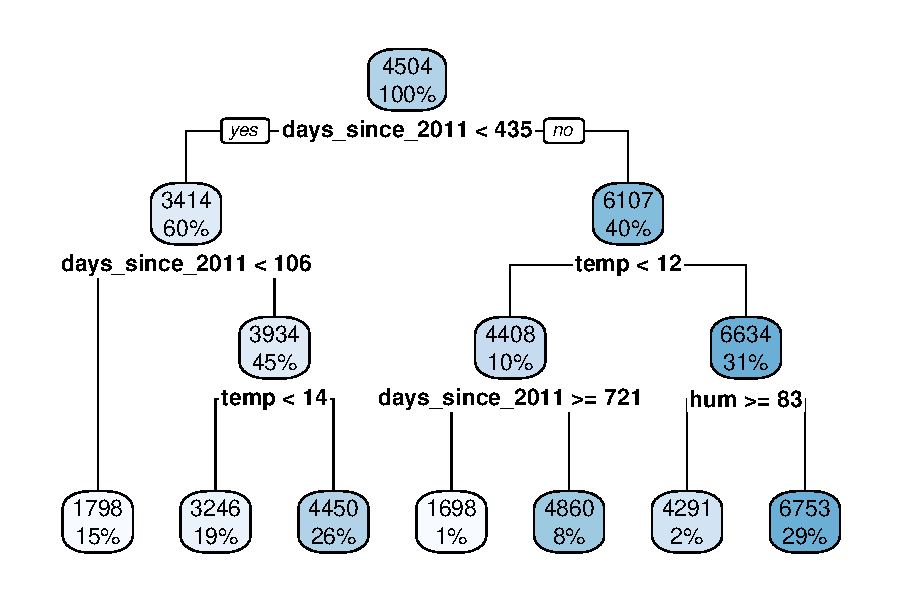
\includegraphics[width = \textwidth]{figure/tree.pdf} 
\end{column}
\end{columns}
 
\end{frame}
%------------------------------------------------------------------
%------------------------------------------------------------------

%\begin{frame}[c]{Decision Rules}

%\texttt{IF COND$_1$ AND COND$_2$ AND ... THEN value}

%\begin{itemize}
%    \item \texttt{COND$_i$} can be of the form \texttt{feature <op> value} where \texttt{<op>} can be for example $\{=, <, > \}$
%\end{itemize}

%\pause
%\medskip

%Properties:
%\begin{description}
%    \item{Support} Fraction of observations to support appliance of rule
%    \item{Accuracy} for predicting the correct class under the condition(s)
%\end{description}

%$\leadsto$ often trade-off between these two

%\pause
%\medskip

%$\leadsto$ many different ways to learn a set of rules (incl. a default rule if none of the rules are met)

%\end{frame}






% %------------------------------------------------------------------
% %------------------------------------------------------------------


% \begin{frame}{Model-based Boosting \citebutton{Bühlmann and Yu 2003}{https://doi.org/10.1198/016214503000125}}

% \begin{itemize}%[<+->]
% %\setlength\itemsep{2em}
% \item<1-> Recall: Boosting iteratively combines weak base learners (BL) %to create a powerful ensemble model
% \item<1->
% Idea: Use simple linear BL to ensure interpretability \\
% %$\leadsto$ e.g., linear BL with single features in each iteration
% %Boosting with gradient descent using interpretable base learners (e.g., use base learners with single features in each iteration $\leadsto$ coordinate gradient descent)
% %The resulting ensemble is also interpretable.
% %\pause
% \item<2->
% Possible to combine linear BL of same type (with distinct parameters $\theta$ and $\theta^{\star}$):
% %Two linear base learners $b_j(x, \theta)$ and $b_j(x, \theta^{\star})$ of the same type, but distinct parameter vectors $\theta$ and $\theta^{\star}$ can be combined in a base learner of the same type:
% $$b_j(x, \theta) + b_j(x, \theta^{\star}) = b_j(x, \theta + \theta^{\star})$$
% %\pause
% \item<3-> %In each iteration, a set of BLs is fitted on pseudo residuals. The one with the best fit is added to the previously computed model (using step-size $\nu$), e.g.,
% In each iteration, fit a set of BLs and add the best BL to previous model (using step-size $\nu$):
% %\medskip
% \begin{align*}
% \widehat{f}^{[1]}(x) &= \hat{f}_0 + \nu \textcolor{blue}{b_3(x_3, \theta^{[1]})} \\
% \visible<4->{\widehat{f}^{[2]}(x) &= \widehat{f}^{[1]}(x) + \nu \textcolor{blue}{b_3(x_3, \theta^{[2]})} 
% %= \hat{f}_0 + \nu \textcolor{blue}{b_3(x_3, \theta^{[1]})} + \nu \textcolor{blue}{b_3(x_3, \theta^{[2]})}
% \\
% \visible<5->{
% \widehat{f}^{[3]}(x) &= \widehat{f}^{[2]}(x) + \nu \textcolor{orange}{b_1(x_1, \theta^{[3]})} 
% %= \hat{f}_0 + \nu \textcolor{blue}{b_3(x_3, \theta^{[1]})} + \nu \textcolor{blue}{b_3(x_3, \theta^{[2]})} + \nu \textcolor{orange}{b_1(x_1, \theta^{[3]})} 
% \\
% &= \hat{f}_0 + \nu \left(\textcolor{blue}{b_3(x_3, \theta^{[1]} + \theta^{[2]})} + \textcolor{orange}{b_1(x_1, \theta^{[3]})}\right) 
% \\
% &= \hat{f}_0 + \textcolor{blue}{\hat{f}_3(x_3)} + \textcolor{orange}{\hat{f}_1(x_1)}
% }
% }
% \end{align*}
% \item<6-> Final model is additive (as GAMs), where each component function is interpretable

% \end{itemize}
% \end{frame}


% \begin{frame}{Model-based Boosting - Example}

% Simple case: Use linear model with single feature (including intercept) as BL
% $$
% b_j(x_j, \theta) = x_j\theta + \theta_0 \hspace*{0.2cm}\text{ for } j = 1,\ldots p \hspace*{0.3cm} \leadsto \text{ordinary linear regression}
% $$

% \begin{itemize}
% \item<1-> Here: Interpretation of weights as in LM
% \item<1-> After many iterations, it converges to same solution as least square estimate of LMs
% \item<2-> Early stopping allows feature selection and might prevent overfitting (regularization)
% %\item Specifying loss and link function according to exponential family leads a (regularized) GLM
% \end{itemize}
% \begin{columns}[T, totalwidth=\textwidth]
% \begin{column}{0.49\textwidth}
% \scriptsize
% \begin{table}[ht]
% \centering
% \begin{tabular}{r|r|l}
%   %\hline
% \textbf{1000 iter. with $\nu = 0.1$} & Intercept & Weights \\ 
%   \hline  \hline
% days\_since\_2011 & -1791.06 & 4.9 \\ 
%   \hline
%   hum & 1953.05 & -31.1 \\ 
%     \hline
%   season & 0 &  \begin{tabular}[c]{@{}l@{}}
%   WINTER: -323.4\\
%   SPRING: 539.5\\
%   SUMMER: -280.2\\
%   FALL: 67.2
%   \end{tabular}\\
%     \hline
%   %season &  & WINTER: -323.4, SPRING: 539.5, SUMMER: -280.2, FALL: 67.2 \\ 
%   temp & -1839.85 & 120.4 \\ 
%     \hline
%   windspeed & 725.70 & -56.9 \\ 
%     \hline
%   offset & 4504.35 &  \\ 
%    %\hline
% \end{tabular}
% \end{table}
% \centering
% $\Rightarrow$ Converges to solution of LM
% \end{column}
% \begin{column}{0.49\textwidth}

% \only<1>{\scriptsize
% Relative frequency of selected BLs across iterations
% 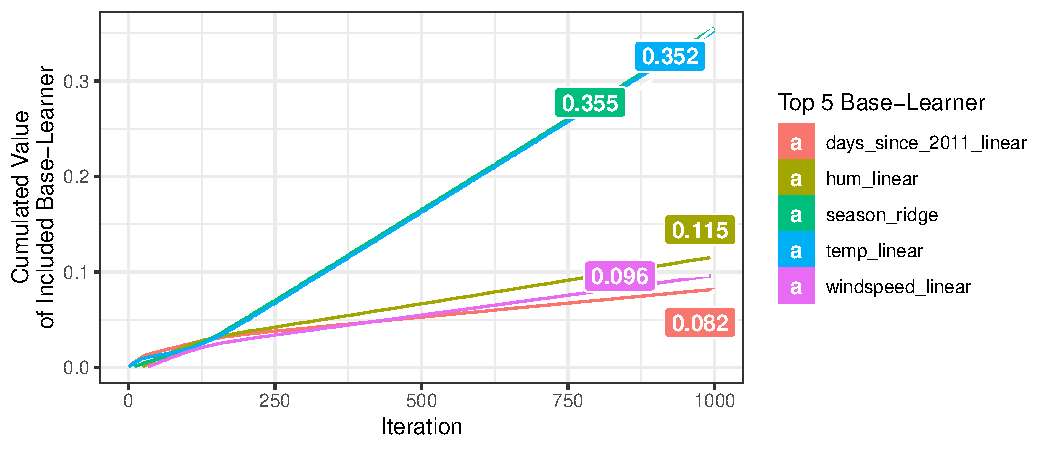
\includegraphics[width = .95 \textwidth]{figure/compboost_base_linear.pdf}}

% \pause
% \scriptsize
% \only<2>{
% \begin{table}[ht]
% \centering
% \begin{tabular}{r|r|l}
%   %\hline
%  \textbf{20 iter. with $\nu = 0.1$} & Intercept & Weights \\ 
%   \hline  \hline
%   days\_since\_2011 & -1210.27 & 3.3 \\ 
%     \hline
%    season & 0 & 
%    \begin{tabular}[c]{@{}l@{}}
%   WINTER: -276.9\\
%   SPRING: 137.6\\
%   SUMMER: 112.8\\
%   FALL: 20.3
%    \end{tabular}\\
%      \hline
%   temp & -1118.94 & 73.2 \\ 
%     \hline
%   offset & 4504.35 &  \\ 
%    %\hline
% \end{tabular}
% \end{table}
% \centering
% $\Rightarrow$ 3 BLs selected after 20 iter. (feature selection)
% }
% \end{column}
% \end{columns}
% % \begin{itemize}
% %     \item Linear base learners for numeric features and categorical base learner for season
% %     \item 3 base learners selected after 100 iterations
% % \end{itemize}
% \end{frame}

% \begin{frame}{Model-based Boosting - Interpretation}

% \begin{itemize}
%     \item Fit model on bike data with different BL types \citebutton{Daniel Schalk et al. 2018}{https://doi.org/10.21105/joss.00967}
%     \item BLs: linear and centered splines for numeric features, categorical for season
%     %and categorical base learner for season
% \end{itemize}
% \begin{columns}[T, totalwidth=\textwidth]
% \visible<2->{
% \begin{column}{0.5\textwidth}
% \hspace{45pt}{\scriptsize{Feature importance}}
%  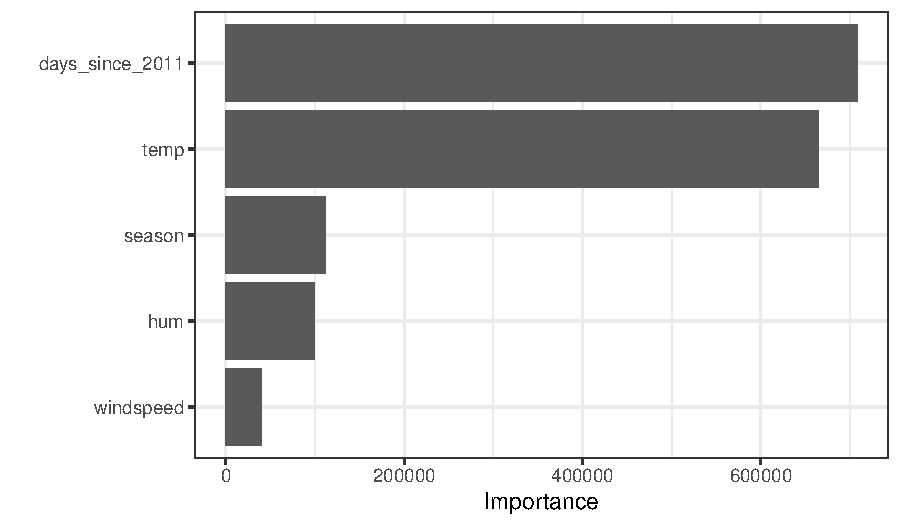
\includegraphics[width = \textwidth]{figure/compboost_pfi.pdf}
% %Feature importance (risk reduction over iter.)\\
% %$\leadsto$ \code{days\_since\_2011} most important
% %\scriptsize
% %\verbatiminput{figure/mboost_output.txt}
% \end{column}
% }
% \visible<3->{
% \begin{column}{0.5\textwidth}  %%<--- here
% \hspace{23pt}{\scriptsize{Feature effect}}
%   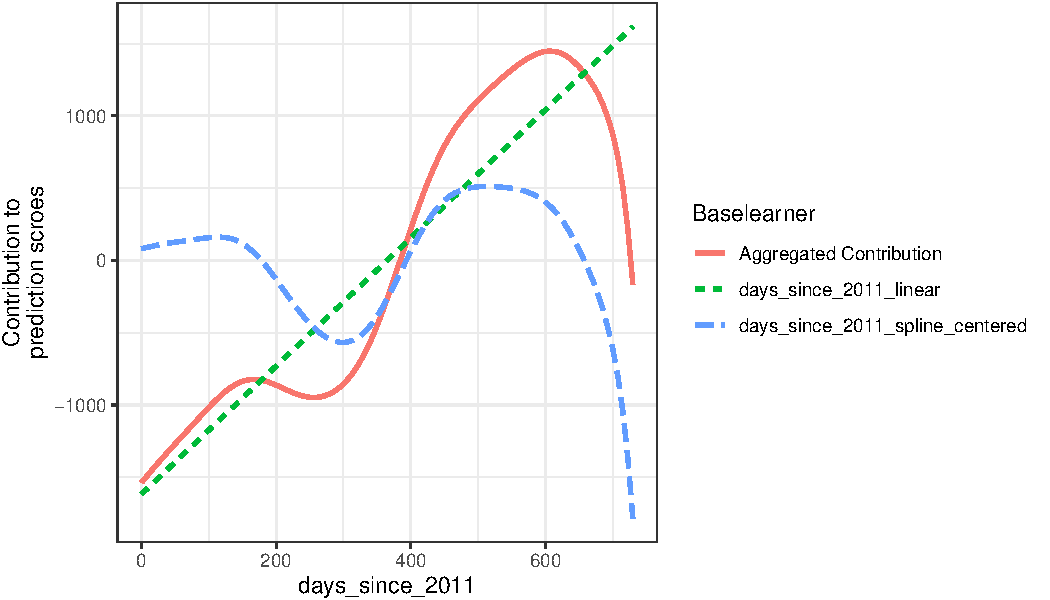
\includegraphics[width = \textwidth]{figure/compboost_pfe.pdf}
% %Partial feature effect for \code{days\_since\_2011}\\
% %$\leadsto$ Total effect: Combination of partial effects of linear BL and centered spline BL
% \end{column}
% }
% \end{columns}
% \begin{itemize}
%     \item<2->  Feature importance (risk reduction over iter.) $\leadsto$ \code{days\_since\_2011} most important
%      \item<3-> Total effect for \code{days\_since\_2011}\\
% $\leadsto$ Combination of partial effects of linear BL and centered spline BL
% \end{itemize}
% \end{frame}


\begin{frame}{Unbiased Recursive Partitioning}  
\vspace{-0.2cm}
\citebutton{Hothorn et al. (2006)}{https://doi.org/10.1198/106186006X133933}
\citebutton{Zeileis et al. (2008)}{https://doi.org/10.1198/106186008X319331}
\citebutton{Strobl et al. (2007)}{https://doi.org/10.1186/1471-2105-8-25}

\vspace{0.2cm}
\textbf{Problems} with CART (Classification and Regression Trees): 

\begin{enumerate}
    \item Selection bias towards high-cardinal/continuous features 
    \item Splits on any improvement, regardless of significance $\leadsto$ prone to overfitting
\end{enumerate}
\smallskip
\pause
\textbf{Unbiased recursive partitioning} via conditional inference trees (\texttt{ctree}) or model-based recursive partitioning (\texttt{mob}): 
\begin{enumerate}  
  \item Separate selection of \textbf{feature used for splitting} and \textbf{split point}
  \item Hypothesis test as stopping criteria 
\end{enumerate}
%\medskip
\pause
\begin{columns}[T, totalwidth = \textwidth]
    \begin{column}{0.5\textwidth}
    \textbf{Example (selection bias)}: \\
         Simulate data ($n = 200$) with $Y \sim N(0,1)$ and 3 features of different cardinality independent from $Y$ (repeat 500 times):
\begin{itemize}
    \item $X_1 \sim Binom(n, \frac{1}{2})$
    \item $X_2 \sim M(n, (\frac{1}{4}, \frac{1}{4}, \frac{1}{4}, \frac{1}{4}))$
    \item $X_3 \sim M(n, (\frac{1}{8}, \frac{1}{8}, \frac{1}{8}, \frac{1}{8}, \frac{1}{8}, \frac{1}{8}, \frac{1}{8}, \frac{1}{8}))$
\end{itemize}
    \end{column}
    \begin{column}{0.5\textwidth}
    \scriptsize
    \centering
    Which feature is selected in the first split?
    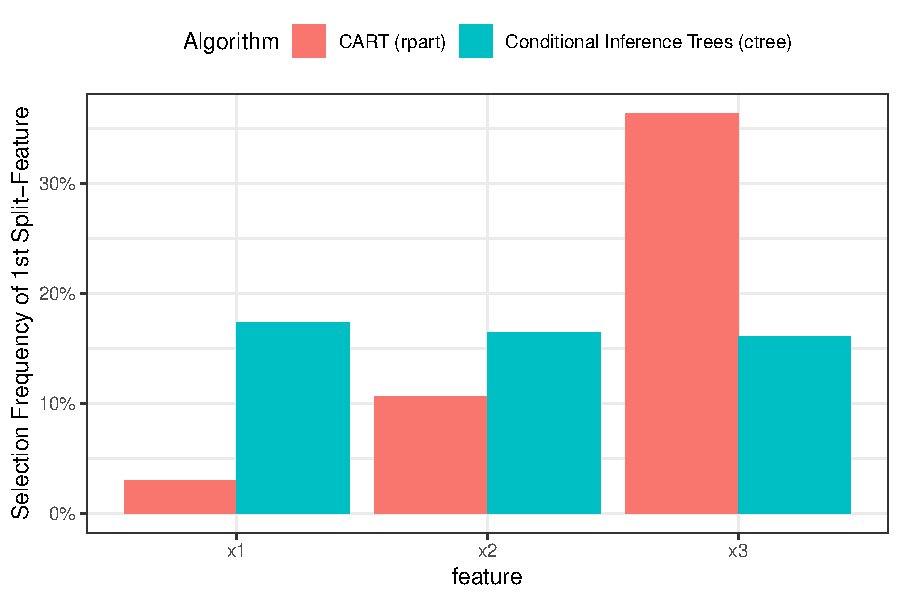
\includegraphics[width = \textwidth]{figure/selection_bias_simulation_1000.pdf}
    \end{column}
\end{columns}
% \medskip
% \scriptsize
% \pause
% \begin{columns}[T, totalwidth = \textwidth]
%     \begin{column}{0.7\textwidth}
%         \textbf{Example (selection bias)}: 
%         $n = 200,\, Y \sim N(0,1)$ \\
%         Simulate features with different cardinality (independent from $Y$):
%         $X_1 \sim N(0,1),\, X_2 \sim B(n, \frac{1}{2},\frac{1}{2}),\, X_3 \sim M(n, rep(\frac{1}{8},8))$
    
%     \medskip
%     \scriptsize{CART decision tree (\texttt{rpart})}\begin{center}
%     \vspace{-0.7cm}
%     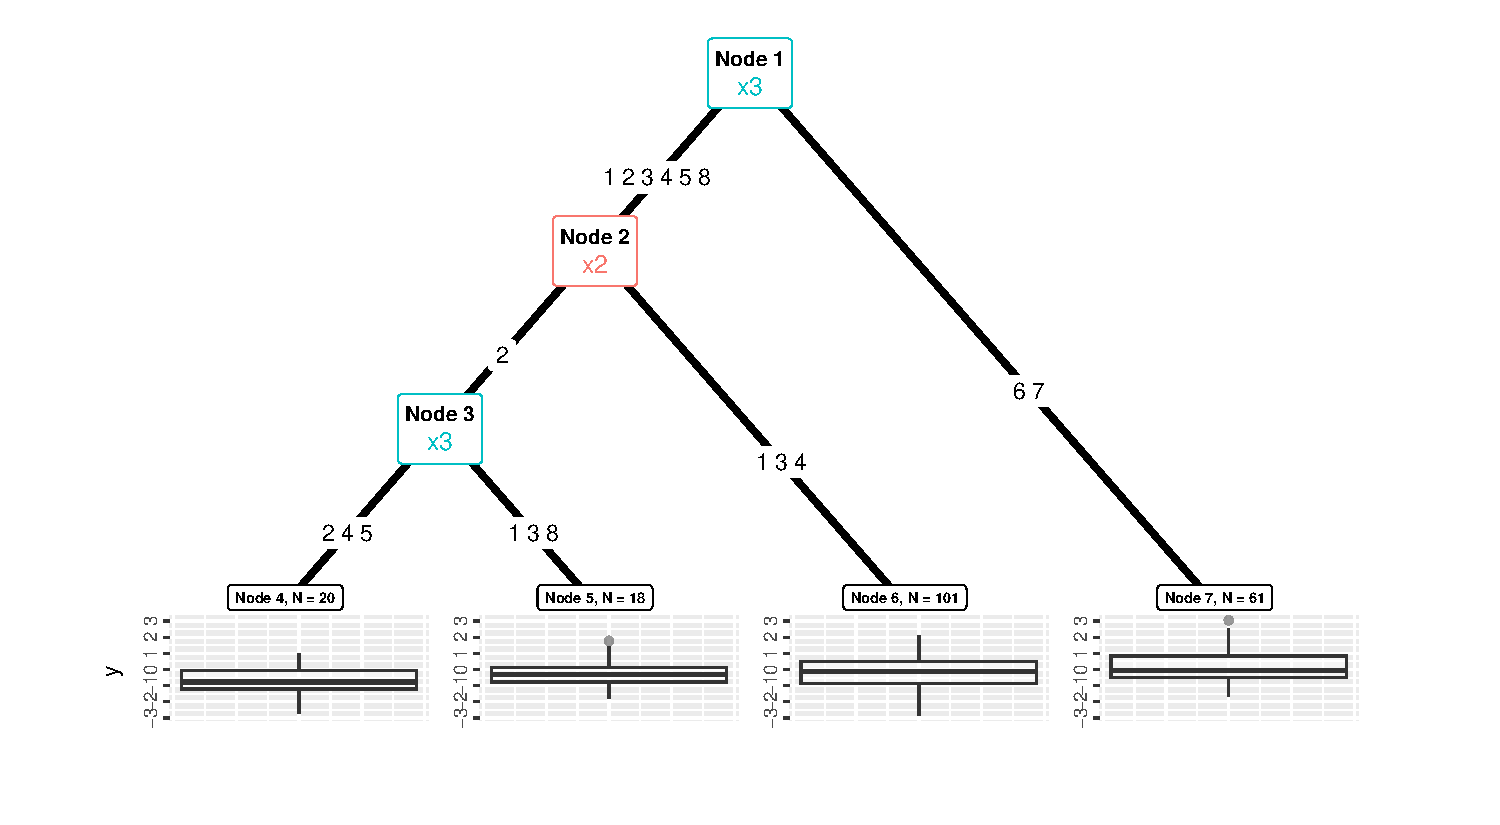
\includegraphics[width = \textwidth]{figure/selection_bias_simulation_tree.pdf}
%     \end{center}
%     \end{column}
%     \pause
%     \begin{column}{0.3\textwidth}
    
%         \textbf{Conditional inference trees}: 
%         \begin{enumerate}  
%         \item Separate selection of feature and split point
%         \item Hypothesis tests as stopping criteria 
%         \end{enumerate}
    
%         \begin{center}
%         \scriptsize{ctree (\texttt{partykit}): 1 node}
%         \vspace{-0.2cm}
%         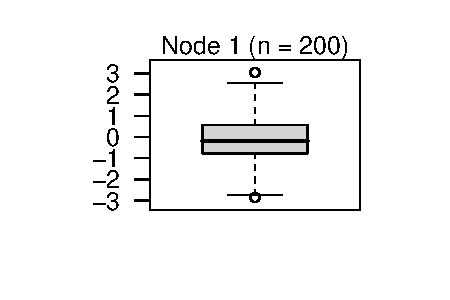
\includegraphics[width = \textwidth]{figure/selection_bias_simulation_ctree.pdf}
%         \end{center}
%         %\normalsize
%     \end{column}
% \end{columns}

\end{frame}


\begin{frame}{Unbiased Recursive Partitioning}

%\vspace{-0.1cm}
Differences to CART:
\begin{itemize}
    \item Two-step approach (1. find most significant split feature, 2. find best split point)
    \item Parametric model (e.g. LM instead of constant) can be fitted in leave nodes % OLS regression, GLMs, and survival regression    
    \item Significance of split (p-value) given in each node
    \item \texttt{ctree} and \texttt{mob} differ in hypothesis test used for selecting the split feature (independence test vs. fluctuation test) and how to find the best split point
\end{itemize}

\medskip

\begin{columns}[c, totalwidth = \textwidth]
     \begin{column}{0.83\textwidth}
\only<2>{
\textbf{Example} (\texttt{ctree}): Bike data (constant model in final nodes)
\centerline{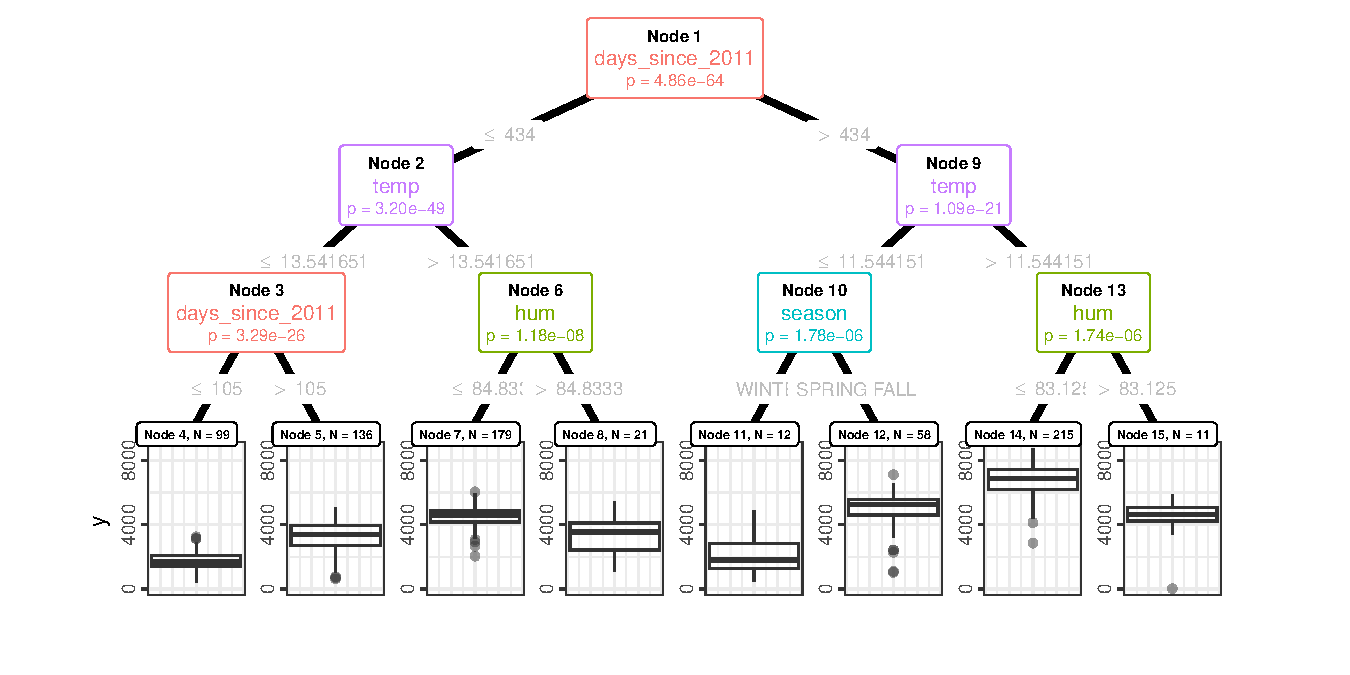
\includegraphics[width =\textwidth]{figure/bike_ctree.pdf}}
}
\only<3>{
\textbf{Example}  (\texttt{mob}): Bike data (linear model with \texttt{temp} in final nodes)
\centerline{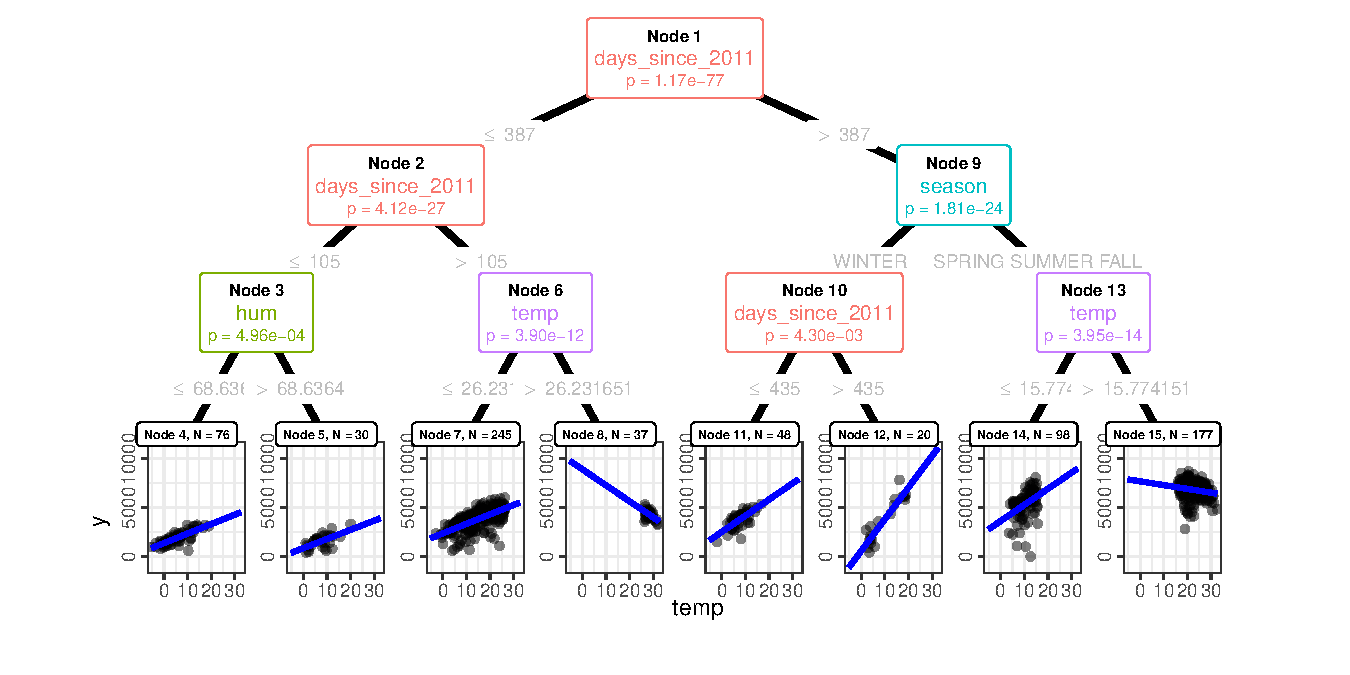
\includegraphics[width = \textwidth]{figure/bike_mob.pdf}}
}
% \only<3>{
% \centerline{Train error (MSE): 758,844.0 (\texttt{ctree}), 742,244.4 (\texttt{mob})}
% }
     \end{column}
     \begin{column}{0.18\textwidth}
     \only<2-3>{\scriptsize
     Train error (MSE): \\
     758,844.0 (\texttt{ctree})\\
     742,244.4 (\texttt{mob})
     }
% \only<3>{
% Comparison MSE: \\
% \texttt{ctree}: 758,844.0 \\
% \texttt{mob}: 742,244.4
% }
     \end{column}
 \end{columns}
\end{frame}


% \begin{frame}{Model-based (MOB) Recursive Partitioning \citebutton{Zeileis et al. (2008)}{https://doi.org/10.1198/106186008X319331}}

% \vspace{-0.1cm}
% \textbf{Idea of MOB}: 

% \begin{itemize}
%     \item If more features are available, the model can be further optimized by considering these new features when partitioning the covariates 
%     \item Advantage: Separation possible, which features to use for splits and which for modeling in leaf nodes
%     \item \texttt{ctree} and \texttt{mob} differ in the variable and split point selection (test statistics)
% \end{itemize}

% \textbf{Example:} Bike data (here: linear model with temp in final nodes)

% \begin{columns}[T, totalwidth=\textwidth]
%     \begin{column}{0.8\textwidth}
% 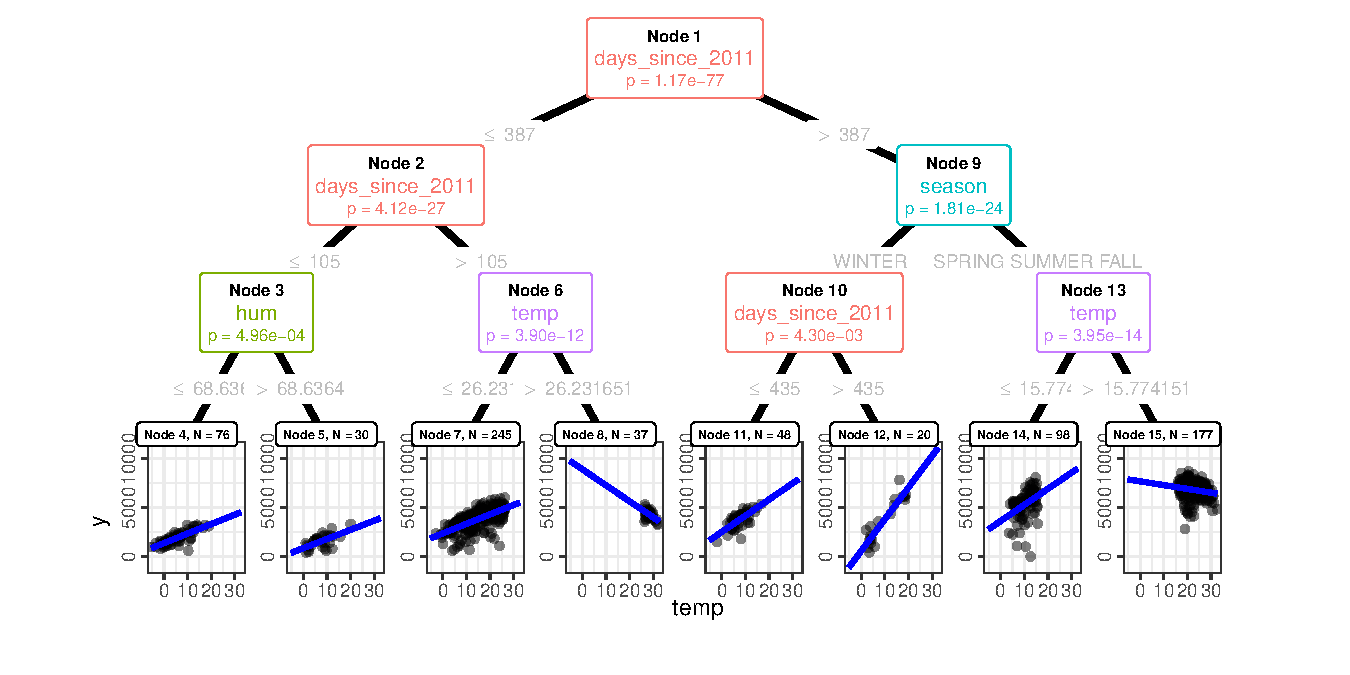
\includegraphics[width = \textwidth]{figure/bike_mob.pdf}
%     \end{column}
%     \begin{column}{0.2\textwidth}
%         \centering
% Comparison RMSE: \\
% \texttt{ctree}: 696,180.7 \\
% \texttt{mob}: 11,994,124.1
%     \end{column}
% \end{columns}
% %\vspace{-0.2cm}



% \end{frame}

%------------------------------------------------------------------
%------------------------------------------------------------------


\begin{frame}[t]{Other Rule-based Models}

\begin{columns}[c, totalwidth=\textwidth]
    \begin{column}{0.6\textwidth}
        \textbf{Decision Rules} \citebutton{Holte 1993}{https://doi.org/10.1023/A:1022631118932}
        \begin{itemize}
            \item Flat list of simple ``if -- then'' statements\\
            $\leadsto$ very intuitive and easy-to-interpret
            \item Mainly devised for classification \\
            (support for regression is limited)
            \item Numeric features are typically discretised
        \end{itemize}
    \end{column}
    \begin{column}{0.4\textwidth}
        %\vspace{\dimexpr-2\parsep-2\parskip\relax}
        %\begin{center}
        \scriptsize
\textcolor{blue}{IF}  $x_{1} \le 2.3$  \textcolor{blue}{AND}  $x_{4} = \text{``A''}$   \hfill\textcolor{blue}{THEN} \hspace{5pt} y = 1\\[2pt]
\textcolor{blue}{ELSE IF}  $x_{2} > 5.0$  \hfill \textcolor{blue}{THEN} \hspace{5pt} y = 2\\[2pt]
\textcolor{blue}{ELSE}  \hfill y = 3
      %  \end{center}
    % \vspace{\dimexpr-2\parsep-2\parskip\relax}
    %     \begin{center}
    %         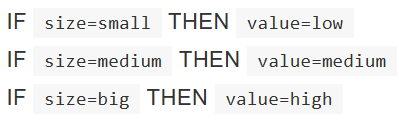
\includegraphics[width = 0.8\textwidth]{figure/decision_rules.png}
    %         % \only<4->{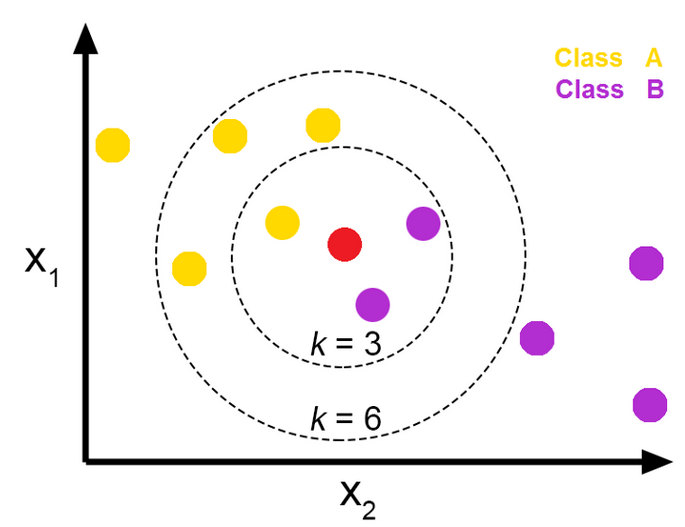
\includegraphics[width = 0.7\textwidth]{figure/knn.png} 
    %         % \citebutton{José 2018}{https://towardsdatascience.com/knn-k-nearest-neighbors-1-a4707b24bd1d}}
    %     \end{center}
    \end{column}
\end{columns}

\bigskip

\begin{columns}[c, totalwidth=\textwidth]
    \begin{column}{0.6\textwidth}
        \only<2->{
        % \textbf{RuleFit} \citebutton{Friedman and Popescu 2008}{https://arxiv.org/abs/0811.1679}
        % \begin{itemize}
        %     \item Combination of LM and decision trees 
        %     \item Uses (many) decision trees to extract important decision rules $r_1, r_2, r_3, r_4$ which are used as features in a (regularized) LM
        %     \item Allows for feature interactions and non-linearities
        % \end{itemize}
        \textbf{RuleFit} \citebutton{Friedman \& Popescu 2008}{https://arxiv.org/abs/0811.1679}
\begin{itemize}
  \item Extract binary rules \(r_m(\mathbf{x}) \in \{0,1\}\) from many shallow trees (one per root-to-leaf path)
  \item Fit an $L_1$-regularized LM
$\hat f(\mathbf x)=\beta_0+\textstyle\sum_m\beta_m r_m(\mathbf x)+\sum_j\gamma_j x_j$
  \item Regularization retains only a few rules\\
  $\Rightarrow$ sparse, non-linear, interaction-aware
  \item Coefficients relate to rule/feature importance
\end{itemize}

        }

        % \only<3->{\textbf{Naive Bayes}
        % \citebutton{Zhang 2004}{https://www.aaai.org/Papers/FLAIRS/2004/Flairs04-097.pdf}
        % %$$P (C_k \mid x ) = \frac{1}{Z} P(C_k) \prod_{i=1}^{n} P(x_i \mid C_k) $$
        % \begin{itemize}
        %     \item Uses Bayes' theorem to assign class prob. to observations
        %     %Product of (conditional) probabilities for a class on the value of each feature
        %     %For each feature, it calculates the probability for a class depending on the value of the feature. 
        %     \item Strong assumption: Independence of features
        % \end{itemize}}

        % \only<4->{\textbf{k-Nearest Neighbor}
        % \citebutton{Cover 1967}{https://doi.org/10.1109/TIT.1967.1053964}
        % \begin{itemize}
        %     \item (Closely related to case-based reasoning)
        %     \item Average of the outcome of neighbors -- local explanation
        % \end{itemize}

        % ...}
    \end{column}
    \begin{column}{0.4\textwidth}
    \vspace{\dimexpr-2\parsep-2\parskip\relax}
        \begin{center}
            \only<2->{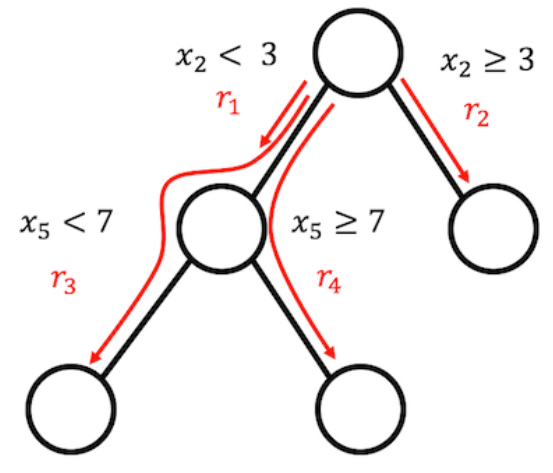
\includegraphics[width = 0.6\textwidth]{figure/RuleFit.png}\\
            \citebutton{Molnar 2022}{https://christophm.github.io/interpretable-ml-book/}\\
            \smallskip }
            % \only<4->{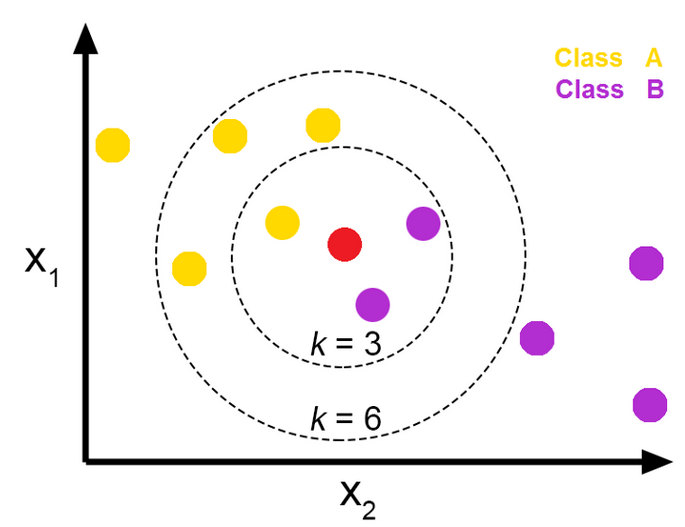
\includegraphics[width = 0.7\textwidth]{figure/knn.png} 
            % \citebutton{José 2018}{https://towardsdatascience.com/knn-k-nearest-neighbors-1-a4707b24bd1d}}
        \end{center}
    \end{column}
\end{columns}
\end{frame}
\endlecture
\end{document}
